\begin{frame}
	\frametitle{Cloudbus Architecture}
	\only<1>{
		\begin{block}{Benefits}
			\begin{itemize}
				\item Cloudbus let developers of distributed applications delegate I/O and other networked IPC decisions to a lower layer.
				\item Cloudbus dynamically controls I/O for application, user ingress, and user egress data.
				\item Cloudbus implements a flexible data routing scheme at the session-layer to enable dynamic data pathway optimizations.
				\item Optimizing I/O in distributed and networked applications offers significant benefits to application performance and reliability.
			\end{itemize}
		\end{block}
	}
	\only<2>{
		\begin{columns}
			\begin{column}{0.7\textwidth}
				\footnotesize
				\begin{itemize}
					\item Users of networked services connect to a controller.
					\item Cloudbus controllers open a cloudbus connection for each user data session.
					\item Controllers service requests by opening 1 or more transport connections towards segments and/or proxies.
					\item Proxies anchor user sessions and provide session state management.
					\item Segments connect to services and expose them into Cloudbus by configuration (DNS or otherwise).					
				\end{itemize}
				\normalsize
			\end{column}
			\begin{column}{0.3\textwidth}
				\begin{figure}
					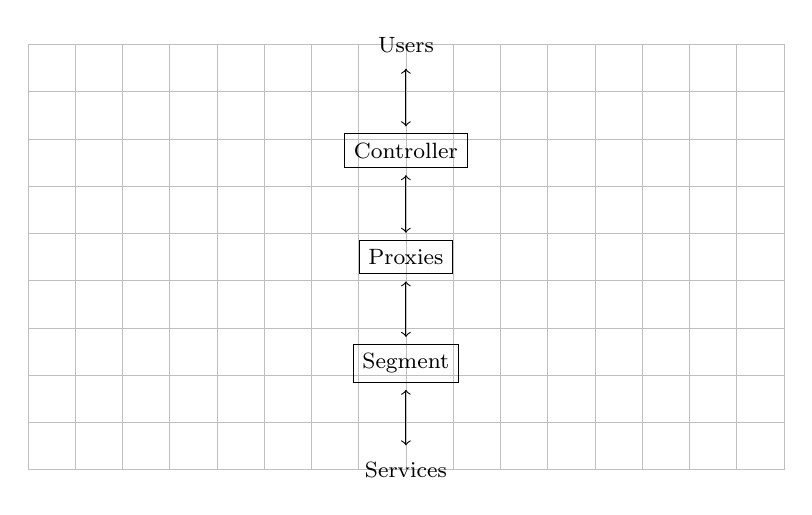
\begin{tikzpicture}[
	scale = 0.6,
	rect/.style={
		rectangle,
		draw=black
	},
	circ/.style={
		circle,
		draw=black
	},
	every node/.style={
		font=\footnotesize
	}
]{
		\def\width{16}
		\def\height{9}
		\draw[help lines, opacity=0.5] (0,0) grid (\width,\height);
		\node(p1) at (8,9){Users};
		\node(c1)[rect] at (8,6.75){Controller};
		\node(pr1)[rect] at (8,4.5){Proxies};
		\node(s1)[rect] at (8,2.25){Segment};
		\node(p2) at (8,0){Services};
		
		\path[<->, shorten >= 0.25em, shorten <= 0.25em] (p1.south) edge (c1.north);
		\path[<->, shorten >= 0.25em, shorten <= 0.25em] (c1.south) edge (pr1.north);
		\path[<->, shorten >= 0.25em, shorten <= 0.25em] (pr1.south) edge (s1.north);
		\path[<->, shorten >= 0.25em, shorten <= 0.25em] (s1.south) edge (p2.north);
}
\end{tikzpicture}\hspace*{5em}
				\end{figure}
			\end{column}
		\end{columns}
	}
	\only<3>{
		\begin{columns}
			\begin{column}{0.5\textwidth}
				\begin{block}{Cloudbus Transport}
					\footnotesize
					\begin{itemize}
						\item Cloudbus encapsulates uniquely identifiable user data streams in session-layer chunks, so it is transport agnostic.
						\item Each chunk is stamped with a UUID, and cloudbus internally routes application traffic using UUIDs instead of the network %
						5-tuple.
						\item Cloudbus treats user session streams as if they are bidirectionally connected (even if the underlying transport is UDP).
					\end{itemize}
					\normalsize
				\end{block}
			\end{column}
			\begin{column}{0.5\textwidth}
				\begin{figure}
					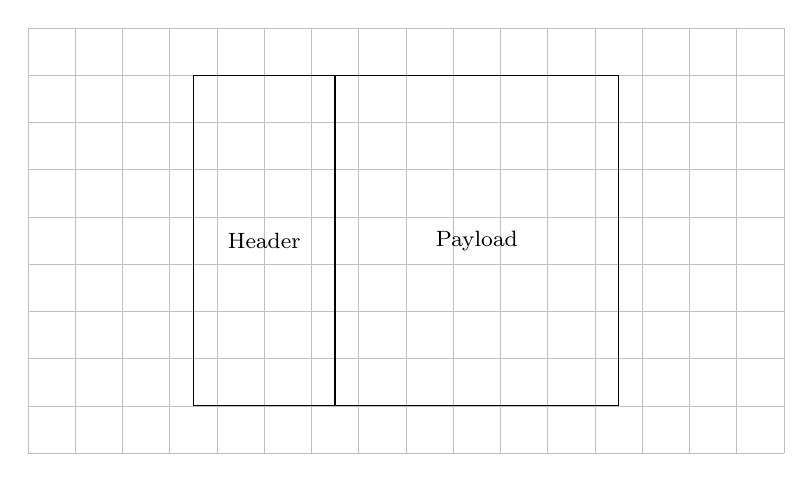
\begin{tikzpicture}[
	scale = 0.6,
	rect/.style={
		rectangle,
		draw=black
	},
	circ/.style={
		circle,
		draw=black
	},
	every node/.style={
		font=\footnotesize
	}
	]{
		\def\width{16}
		\def\height{9}
		\draw[help lines, opacity=0.5] (0,0) grid (\width,\height);
		\draw (3.5,1) rectangle (6.5,8);
		\node at (5, 4.5){Header};
		\draw (6.5,1) rectangle (12.5,8);
		\node at (9.5,4.5){Payload};	
	}
\end{tikzpicture}
					\caption{Cloudbus data encapsulation}
				\end{figure}
			\end{column}
		\end{columns}

	}
\end{frame}